\chapter{Lexical Entailment in RTE}
\label{ch:rte}

This chapter how the work of the previous three chapters may be combined into
an end-to-end RTE system, and related material. Some of the results in this
chapter have been published in \newcite{beltagy:2016:cl}. Contributions
of the dissertation author are layed out in this text.

\section{Chapter Overview}

In the previous chapters, we showed how improvements in modeling can lead
to better performance in several lexical tasks, including lexical relationship
prediction, lexical entailment detection, and lexical substitution. Each of
these tasks is valuable in its own right, but it is important not to lose
sight of the bigger picture. We turn our attention now to the Recognizing
Textual Entailment task (RTE), which we introduced in the beginning of
Chapters~\ref{ch:intro}~and~\ref{ch:background}.

In the RTE, a system is provided two sentences, a text (antecdent) and
hypothesis (consequent), and must decide whether the text logically
entails the hypothesis.
A particular RTE pair may involve different logical conclusions, but
\newcite{dagan:2006:mlc} observed that lexical entailments are often critical
to reaching the proper conclusion. In our original example, we saw a mix of
several aspects of lexical entailment examined in this thesis, including
hypernymy, polysemy, and event understanding:
\begin{quote}
  \label{ex:rte}
  Text: The bright girl reads a book.\\
  Hypothesis: A smart child looks at a book.
\end{quote}
Given the importance of lexical entailment in the RTE task, we expect that
the contributions from previous chapters should be reflected in an end-to-end
RTE system. We begin with a brief expository into the RTE system we use, and
then integrate our contributions in directly.

\section{RTE System}
\label{sec:rtesystem}

We use the RTE system of \newcite{beltagy:2016:cl} to evaluate our improvements
in lexical entailment. Although this dissertation author is also a co-author on
that paper, this section (\ref{sec:rtesystem}) primarily describes efforts of
others, and should not be seen as a contribution of this thesis. In short,
this section explains the RTE system at an abstract level, and considers how it
reduces sentences into lexical entailment subproblems. We do not review other
systems for RTE, as most approaches were outlined in
Section~\ref{sec:textent}, and their differences are not the focus of this
document.

The RTE system of \newcite{beltagy:2016:cl} works on a principal of textual
entailment using {\em probabilistic} logical deduction. In principal, it
computes a First Order Logical (FOL) representation of each sentence, and
then attempts to compute the probability that the second sentence is entailed
using probabilistic logic using a probabilistic logic formalism called
Markov Logic Networks (MLNs) \cite{richardson:2006:ml}. MLNs take as input a
knowledge base of facts about the world in the form FOL formulas (including
atomic formulas), and compute the probability of a given formula using a
graphical model. The probability of a formula being true is exponential the
number of facts it is consistent with. This powerful formulation is outside
the scope of this document, but with careful consideration, MLNs are able
to model a large variety of natural language phenomena, including
quantifiers and negation \cite{beltagy:2016:phd}.

However, in order to perform correct logical reasoning, the system must reduce
the text and hypothesis into logical formulas, and consider a database of
relevant facts. To obtain a logical representation of the sentences, the
RTE system employs Boxer \cite{bos:2008:step}, which converts syntactic parse
trees into neo-Davidsonian logical formulas \cite{parsons:1990:events}. In our
original example from the Overview, Boxer would produce roughly:
\begin{align*}
  \mbox{Text:}~\exists g,r,b.[ & girl(g) \wedge bright(g) \wedge read(r) \\
                               & \qquad \wedge agent(r, g) \wedge patient(r, b) \wedge book(b)]\\
  \mbox{Hypothesis:}~\exists c,l,x.[ & child(c) \wedge smart(c) \wedge look\_at(l) \\
                               & \qquad \wedge agent(l, c) \wedge patient(l, x) \wedge book(x)]
\end{align*}

The RTE system then performs a form of Robinson Resolution or Unification on
the two sentences, in order to obtain a list of {\em possible} lexical
entailments. In the simple running example, we would observe that \lit{book}
appears in both sentences, and assume that it is coreferent across both
sentences. Although coreference may not be strictly assumed in true logical
entailment, it is frequently assumed by annotators of natural language
entailments \cite{marelli:2014:semeval,bowman:2015:emnlp,beltagy:2016:cl}.
This allows the $book(b)$ and $book(x)$ subexpressions to be unified, and
these subexpressions can then be removed, and the logical forms may
be simplified: 
\begin{align*}
  \mbox{Text:}~\exists g,r,b.[ & girl(g) \wedge bright(g) \wedge read(r) \wedge agent(r, g)]\\
  \mbox{Hypothesis:}~\exists c,l,x.[ & child(c) \wedge smart(c) \wedge look\_at(l) \wedge agent(l, c)]
\end{align*}

Similarly, event variables are also assumed to be coreferent
\cite{bowman:2015:emnlp,beltagy:2016:cl}, so we assume that the \lit{read}
event and the \lit{look at} events are aligned, though we do {\em not} assume
they are necessarily entailed. By process of elimination, the $g$ and $c$ variables
must be also aligned, and so this RTE problem has been reduced to two
lexical entailments:
\begin{align*}
  \mbox{bright girl} & \rightarrow \mbox{smart child}\\
  \mbox{read} & \rightarrow \mbox{look at}
\end{align*}
The RTE system then queries a lexical entailment system to predict whether
these lexical items are entailed, neutral, or contradictory. These lexical
entailment predictions are finally encoded as facts about the world, and
complete probabilistic logical reasoning is performed about the full sentences
(including quantification and negation), and a final decision about sentence
entailment is decided.

\section{RTE Data and Lexical Entailment Annotations}

We evaluate using the Sentences Involving Compositional Knowledge (SICK)
dataset, which contains nearly 10k sentence pairs, evenly split between
training and test sets \cite{marelli:2014:semeval}. Sentence pairs were
extracted randomly image caption datasets, and then simplified and extended to
cover semantic issues like negation, quantification, compositional language,
and a variety of lexical entailment relationships like hypernymy and polysemy.
Finally, sentences were manually annotated as {\em entailing} (the antecedent
implies the consequent), {\em contradicting} (the antecedent implies the
opposite of the consequent), or neutral (neither of the above). SICK's
construction makes it an excellent dataset to test a complete RTE system, due
to the rich variety of semantic phenomena it covers. Two examples from the
dataset are shown in Table~\ref{tab:sickexample}.

\begin{table}
  \centering
  \begin{tabular}{|ll|}
    \hline
    {\bf Label} & {\bf Antecedent/Consequent}\\
    \hline
    Entailing & A: Two teams are competing in a football match\\
    & C: Two groups of people are playing football\\
    \hline
    Contradicting & A: The brown horse is near a red barrel at the rodeo\\
    & C: The brown horse is far from a red barrel at the rodeo\\
    \hline
  \end{tabular}
  \caption{Example entailing and contradicting sentences from the SICK dataset.}
  \label{tab:sickexample}
\end{table}

We saw above that we may break some sentences down into
individual lexical entailments of small or short phrases. These lexical
entailments may be either entailing, neutral, or contradicting. This differs
from work in previous chapters, where we focused only on lexical substitution,
identifying what relationship a pair of words exhibits, or treating entailment
as a binary decision. Here, we must provide lexical entailments which are
tailored directly for the RTE task at hand, and so we must build a lexical
entailment dataset.

To do this, we used the Robinson Resolution approach described above to extract
all the lexical entailments possible in the system. Many of these lexical
entailments could be automatically annotated from the RTE sentences themselves:
if the sentence is entailing and contains no negation, it follows that the
individual lexical entailments must also entail. This allows us to build a list
of certainly true lexical entailments. Sentences that are contradicting and
contain only a single lexical entailment rule, can similarly have their lexical
entailments automatically labeled as contradicting. Sentences which are neutral
or contain certain logical phenomena may {\em not} be automatically annotated.
For these sentences, two authors of \newcite{beltagy:2016:cl} (including this
dissertation's author) manually annotated ambiguous lexical entailment pairs
derived from the dataset. We only annotated lexical entailment pairs derived
from the training set, as we did not want pairs from the test set to possibly
influence our decisions, and any lexical annotations derived from the test set
would be considered cheating. The final lexical entailment dataset contains
10,213 annotated rules extracted from the SICK training set.

\section{Lexical Entailment Classifier}

We now turn our focus to the actual lexical entailment classifier used by the
RTE system. This lexical entailment classifier employes a variety of techniques
used in prior work, as well as novel contributions. As a starting point for
the classifier, we employ a wide variety of hand-engineered features
shown by \newcite{lai:2014:semeval} to be useful in the SICK dataset. These
features are given to a basic SVM classifier with an RBF kernel, which
decides which of the three lexical entailment decisions to make. We also
employ a greedy alignment procedure which allows the lexical entailment
classifier to classify short phrases as opposed to single words.
Finally, describe additional features for the lexical entailment classifier
based on our findings about supervised distributional lexical entailment
classifiers, and lexical substitution.

\subsection{Baseline Features (Lai and Hockenmair~(2014)}

The baseline set of features we use were originally proposed by
\newcite{lai:2014:semeval}, and consist of basic phrase features
(e.g. lengths of the phrases), wordform features (e.g. do these words
carry the same lemma or POS?), WordNet features (e.g. are these two words
hypernyms in WordNet), and distributional features (e.g. cosine similarity).
A full list of these features may be found in Table~\ref{tab:lexentfeat},
along with their types and counts.

The Wordform features include simple features like are the words of the same
part-of-speech, same lemma, which are singular/plural, and so forth. On their
own, they can only capture the most simple entailments and slight prior
information. Similarly, the basic alignment features contain only information
like length of the LHS and RHS, and that difference, and which is generally
semantically void, but does inform entailment priors.

The Distributional features contain simple cosine similarities for the LHS and
RHS using one syntactic distributional space and one bag-of-words
distributional space.
The syntactic distributional space is comparable
to the one used in the previous sections, and was trained in roughly the same
preprocessing as in Chapter~\ref{ch:hpm}: part-of-speech tagged, lemmatized,
collapsed-dependencies, PPMI-transformed and SVD reduced to 300 dimensions.
The BoW distributional space is a standard Word2Vec space, trained with
a window size of 20 using the same preprocessed corpus as the syntactic
space. We choose the large BoW window so that the dependency and BoW spaces
would measure each extreme of the function-topic similarity spectrum.

Finally, the WordNet features are the most sophisticated, and contain simple
extractions of WordNet relationships: whether the LHS and RHS are listed as
synonyms, antonyms, or hypernyms of each other (directly or across a long
chain) in WordNet. Additionally, the Path Similarity is also included, as
implemented by \newcite{bird:2009:nltk}.



\begin{table}
\centering
\begin{small}
\begin{tabular}{|lllr|}
    \hline
    \bf{Name} & \bf{Description} & \bf{Type} & \bf{\#}\\
    \hline\hline
    \multicolumn{3}{|l}{\bf{Simple alignment Features}} & 10 \\
    \hline
    Length & Length of LHS, RHS and (absolute) difference & Real & 4\\
    Alignments & Number of aligned/unaligned words on LHS and RHS & Real & 3\\
    Align Pct. & Alignment statistics rescaled to percentages & Real & 3\\
    \hline\hline
    \multicolumn{3}{|l}{\bf{Wordform}} & 18\\
    \hline
    Same word & Same lemma, surface form & Binary & 2\\
    POS & POS of LHS, POS of RHS, same POS & Binary & 10\\
    Sg/Pl & Whether LHS/RHS/both are singular/plural & Binary & 6\\
    \hline
    \hline
    \multicolumn{3}{|l}{\bf Distributional features} & 28\\
    \hline
    OOV & True if either lemma not in dist space & Binary & 2\\
    BoW Cosine & Cosine between LHS and RHS in BoW space & Real & 1\\
    Dep Cosine & Cosine between LHS and RHS in syntactic space & Real & 1\\
    BoW Hist & Bins of BoW Cosine & Binary & 12\\
    Dep Hist & Bins of Dep Cosine & Binary & 12\\
    \hline
    \hline
    \multicolumn{3}{|l}{\bf WordNet} & 18\\
    \hline
    OOV & True if a lemma is not in WordNet, or no path exists & Binary & 1\\
    Hyper & True if LHS is hypernym of RHS & Binary & 1\\
    Hypo & True if RHS is hypernym of LHS & Binary & 1\\
    Syn & True if LHS and RHS is in same synset & Binary & 1\\
    Ant & True if LHS and RHS are antonyms & Binary & 1\\
    Path Sim & Path similarity (NLTK) & Real & 1\\
    Path Sim Hist & Bins of path similarity (NLTK) & Binary & 12\\
    \hline
\end{tabular}
\caption{List of baseline features in the lexical entailment classifier, along
with types and counts. Most of these were proposed by Lai and Hockenmaier~(2014),
with the exception of the Binning features.}
\label{tab:lexentfeat}
\end{small}
\end{table}

\subsection{Alignment Features (Lai and Hockenmaier, 2014)}
\label{sec:alignment}

Since the lexical entailments that we are provided may possibly be short
{\em phrases} rather than individual words, we also use a variation of the
alignment procedure proposed by \newcite{lai:2014:semeval}. In this alignment
procedure, the syntactic head of the phrases are assumed to be aligned, and
the baseline features are computed between the heads of the LHS and RHS.
The remaining words are then greedily aligned using distributional similarity:
the distributional similarity between the every non-head word on the LHS and
RHS is computed, and then the distributionally most similar pair is assume to
be aligned and removed from the pool of unaligned words. This process is
recursively repeated until one or both phrases has all its words exhausted.
Finally, the hand-engineered features described in Table~\ref{tab:lexentfeat}
are then computed for all the aligned pairs, and a min/mean/max of all the
features across all aligned pairs is computed and used as additional features
for the lexical entailment classifier. Since phrases may have been extracted
from neutral sentences, sometimes the alignments may be very poor, but these
bad alignments will be reflected in the statistics and learned as nonentailing
by the classifier.

\subsection{Binning of Similarity Features}

The features and alignment procedure described above are primarily derived
from the observations of \cite{lai:2014:semeval}, who won the original shared
task for this dataset. However, we do include one novel addition to
these features which was not proposed in prior work, which we call
{\em similarity binning}. We extend the real-valued distributional-similarity
features by {\em binning} the cosine similarities into discretized ranges
(e.g. 0.0--0.1, \ldots, 0.9--1.0), and transforming them into binary-valued
indicator features. This stems from an observation that the probability of
entailment is non-monotonic in distributional similarity.

We can observe this fact in Figure~\ref{fig:valley}, which shows the
distribution of entailment annotations as a stacked histogram over
distributional similarities. Observe that
mid-similar terms (those with a cosine of $\sim.80$, like {\em cat} and {\em
animal}) are more likely entailments than those with high similarity
(cosine of $\sim.95$, like {\em cat} and {\em dog}). We found this binning
technique significantly improved the contribution distributional similarity
in feature-engineered lexical entailment classifiers, and this binning
represents a contribution of this thesis. We will visit the effect of binning
in the Experiments section.

\begin{figure}
  \centering
  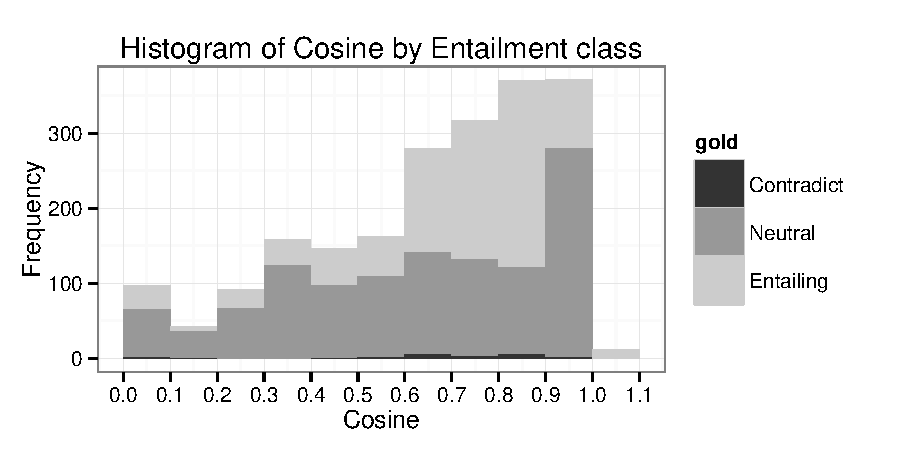
\includegraphics[width=0.90\textwidth]{plots/valley.pdf}
  \caption{Distribution of entailment relations on lexical items by cosine.
    Highly similar pairs (0.90--0.99) are less likely entailing than moderately
    similar pairs (0.70--0.89).}
  \label{fig:valley}
\end{figure}

\subsection{Distributional Classifiers}

We also include several variations of features from the Supervised
Distributional Lexical Relationship classifiers of Chapters \ref{ch:lexmem} and
\ref{ch:hpm}. Namely, we consider and compare three main models:
\begin{itemize}
  \item {\bf Concat}: We include the vectors representing the head word of the
    LHS phrase and the head word of the RHS phrase, unit-normalized. This
    corresponds to the RBF model from Table~\ref{tab:results}, since the
    baseline classifier uses an RBF kernel.
  \item {\bf Asym}: We include the vector difference and vector difference
    between the LHS and RHS head words, like the model explored in
    Chapter~\ref{ch:lexmem}. Note that since the classifier uses an RBF kernel,
    this is slightly different than our original Asym classifier. However,
    we tested both and found the difference was marginal.
  \item {\bf H-features}: We follow the H-feature extraction procedure described
    in Chapter~\ref{ch:hpm} and extract several iterations of H-features
    for the LHS and RHS head words. This is directly comparable to the
    H-feature model.
\end{itemize}
Ideally, we should see that the inclusion of these models should provide
additional, useful information for the lexical entailment classifier, similar
to our findings in the previous chapters. Note that we do not try additional
Distributional classifiers, like the Ksim model of \newcite{levy:2015:naacl},
due to the requirement that the models integrate cleanly with the baseline
features. We also note these features are {\em not} combined with the
alignment procedure (Section~\ref{sec:alignment}), as this would increase
the number of features to be much larger than the number of labeled examples.

Since we are the first to use these supervised distributional features in any
sort of lexical entailment classifier for RTE, all three should be considered
original contributions.

\subsection{Context Vector Features}

Finally, we also include {\em context} similarity features, inspired by the
addCos \cite{melamud:2015:vsm} and nPIC \cite{roller:2016:naacl} models of
Lexical Substitution discussed in Chapter~\ref{ch:lexsub}. These context
similarity features required modification of the lexical substitution models,
as naive application of either did not produce positive results. Additionally,
since we are the first to include context similarity features into the RTE
task, these features are an additional contribution of this thesis.

For each pair of head words on the LHS and RHS, we extract all syntactic
contexts from the original pair of sentences, and look up their respective {\em
context} vectors from the Context matrix learned by the syntactic
distributional space. We then measure five similarities arising
from the possible combinations contexts and words:
(1) context of LHS with RHS head, (2) context of RHS with LHS head,
(3) context of LHS with LHS head, (4) context of RHS with RHS head, and
(5) context of LHs with context of RHS.

The first feature is the cosine similarity between the syntactic contexts of
the LHS agree with the RHS. This measures how well the RHS's selection
preferences agree with the LHS. The reverse corresponds to our
second similarity. Based on the findings of Chapter~\ref{sec:lexsub}, these
features correspond roughly to how well the RHS serves as a substitute in
the LHS, and vice versa. These features are mostly directly analogous to the
addCos model of \newcite{melamud:2015:vsm}; we also tried {\em unnormalized}
inner products similar to the PIC model, but we found simple cosine performed
better.

The third and fourth similarities (LHS contexts with LHS head, RHS contexts
with RHS head) do not have an analogous relationship to lexical substitution.
However, their purpose is quite intuitive: if the LHS does not strongly agree
with its context, then neither should any of its lexical substitutes. In this
way, these agreement features do not inform the lexical entailment
classifier, except in setting a level of importance for the lexical substitution
features.

The final, fifth feature is the similarity between the contexts from the LHS
and the contexts of the RHS. This has no relationship to the lexical
substitution models, but we found it was important for strong, robust results.
This feature works by ensuring that the contexts of the LHS and RHS are
similar, and most readily captures tricky RTE phenomenon like subject-object
reversal.  For example, this feature will identify that the role of \lit{man}
in \lit{dog bites man} differs substantially from its role in \lit{man bites
dog}. This sort of argument-reversal is one important RTE phenomena which
is traditionally ignored in simple alignment and distributional models.

\section{Experiments and Results}

We evaluate all models in two experimental settings, both derived from the
Sentences Involving Compositional Knowledge (SICK) dataset, which contains
approximately 5000 training and 5000 testing sentence pairs. In the first
setting, we evaluate {\em only} the lexical entailment classifier on its
ability to correctly identify lexical pairs as entailing, contradicting or
neutral. In this setting, we evaluate only on the lexical entailment rules
extracted using the Unification procedure described in
Section~\ref{sec:rtesystem}. Since only the lexical rules from the training set
are annotated, this evaluation is uses a 10-fold cross validation setting.  No
validation set is used, but hyperparameters were tuned by maximizing
performance across all 10 folds; however, since we are only evaluating on the
training set, it is fair to optimize hyperparameters in this way. This
experimental setup does not involve the RTE system in any way, and performance
is measured in accuracy.

In the second experimental setup, the lexical entailment classifier is trained
using all rules extracted from the training set, and then applied to all
lexical pairs extracted from the testing set; since the lexical rule extraction
procedure is unsupervised, this is the proper way to test generalization to the
RTE test set. These test-set lexical predictions are then provided to the RTE
system, and the RTE system makes final predictions for the RTE test set. These
predictions are evaluated on the RTE dataset directly, so they test how well
each of the lexical entailment models contribute as information sources in the
logical RTE system. Though the original system described in
\newcite{beltagy:2016:cl} uses several resources of world knowledge and
additional heuristics, in these
experiments the lexical entailment classifiers are the {\em only} source of
knowledge. These results are also measured in accuracy.

We emphasize that we do {\em not} test any of these models
in a zero lexical overlap setting. In the experiments of previous chapters, our
goal was to test generalization to new lexical items; in these experiments, our
goal is to generalize to new RTE examples. Therefore, all of the sentence pairs
will be unique, but will involve many non-unique lexical entailments: for
example, the pair (man, woman) appears frequently in both training and test.

\subsection{Individual Components}

We first compare each of the individual components of the lexical entailment
classifier as how they perform alone, as the single source of lexical
knowledge. We also consider one lower and one upper baseline model: the lower
baseline model is a majority baseline which always guesses ``neutral,''
so its performance on the RTE Test set can be considered the performance
of the {\em logical system alone}. The upper baseline is given the gold
labels for every example, and so its Lexical score is a perfect 100\%,
but its RTE test score is not; this represents the most any lexical classifier
alone can contribute, and any remaining performance is due to inconsistent
labeling, errors in logical conclusions, incorrect parsing, or any other
imperfections in the end-to-end RTE system.
Additionally, we include each of the four sets of features obtained from
the work of \newcite{lai:2014:semeval}, as comparison points. Finally, we
compare each of the our original contribution modules. 

\begin{table}
  \centering
  \begin{tabular}{|lrr|}
  \hline
  {\bf Model}                & {\bf Lexical} &     {\bf RTE}  \\
  \hline\hline
  Neutral (lower baseline)    &      .643     &        .735   \\
  Gold (upper baseline)       &     1.000     &        .968   \\
  \hline
  Simple alignments           &      .643     &        .735   \\
  Wordform features           &      .676     &        .766   \\
  Distributional (no binning) &      .678     &        .758   \\
  WordNet                     &      .754     &        .815   \\
  \hline
  \multicolumn{3}{c}{}\\
  [-0.5em]
  \multicolumn{3}{c}{(a) Baseline features}\\
  \multicolumn{3}{c}{}\\
  \hline
  {\bf Model}                & {\bf Lexical} &     {\bf RTE} \\
  \hline\hline
  Distributional (w/ binning) &      .714     &        .770   \\
  %\hline
  %\multicolumn{3}{c}{}\\
  %\hline
  %\multicolumn{3}{|c|}{{Context Features}}\\
  \hline
  %\multicolumn{3}{c}{}\\
  %\hline
  %\multicolumn{3}{|c|}{{Supervised Relationships}}\\
  %\hline
  Concat (RBF)                &      .716     &        .788   \\
  Asym                        &      .703     &        .777   \\
  H-features                  &      .716     &        .784   \\
  \hline
  Context features            &      .691     &        .764   \\
  \hline
  \multicolumn{3}{c}{}\\
  [-0.5em]
  \multicolumn{3}{c}{{(b) Original Contributions}}\\
  \end{tabular}
  \caption{Comparison of individual lexical entailment components on the.}
  \label{tab:indivrte}
\end{table}

The results of all these models may be seen in Table~\ref{tab:indivrte}.
We first observe that the Gold lexical baseline has a nonperfect score
on RTE test, marking the ceiling of contributions from any of our models, and
that it is considerably higher than the lower baseline. This is consistent
with the observations of \cite{dagan:2006:mlc}, who found Lexical Entailment
to be an important component of any RTE system.

We also observe that the strongest individual component, by a large margin, is
the WordNet features. This is not surprising, as WordNet is a large,
comprehensive and high-quality resource. Additionally, most of the words in SICK
contain WordNet entries, and many of SICK's entries specifically cover
simple hypernymy.

We also observe that the Supervised Distributional features substantially
outperform the baseline features, with the exception of WordNet. This is
consistent with our findings in previous chapters: simple cosine similarity
alone is not enough to detect entailment
\cite{weeds:2004:coling,baroni:2012:eacl,lenci:2012:starsem}, and there is
great deal of benefit using the full distributional vectors in an entailment
classifier
\cite{roller:2014:coling,kruszewski:2015:tacl,roller:2016:emnlp,shwartz:2016:acl}.
Somewhat surprisingly, we find that the Concat and H-features models both
perform the same in the Lexical evaluation, but Concat slightly outperforms
H-features in the end-to-end RTE evaluation. This emphasizes one important
difficulty in using Lexical classifiers in RTE evaluation: many sentence pairs
require observing {\em several} correct lexical entailments to reach the
correct, final conclusion. Therefore, small improvements in the lexical
entailment classifier may not translate to improvements in the RTE dataset.

We also see that adding the binning to the distributional features
substantially improves both the Lexical evaluation and RTE evaluation, compared
to the baseline distributional features without binning. In fact, this simple
technique brings the distributional similarity classifier to nearly the quality
as some of our supervised distributional models. This conforms to our
observation in Figure~\ref{fig:valley} and emphasizes that a larger context
is important , which found that the conditional
probability for entailment differs across different similarity levels.

Finally, we see that the Context features based on Lexical Substitution
also outperforms many of the individual baseline features, including
the distributional features (without binning). This emphasizes that integrating
a wider context is important in lexical entailment, and that lexical
entailment should not be considered in a vacuum.

In the next section, we will combine each of our contributions and consider
whether our models may improve upon the Baseline features of prior work,
as well as the strengths and weaknesses of our components.

\subsection{Combining Components}

Each of our contributing components discussed above are roughly orthogonal
in purpose: binning should capture different entailment liklihoods for
different distributional similarities; Context features should capture
polysemy or changes in larger context; and Supervised Distributional features
should improve generalization to new lexical pairs. Each component should
combine to improve overall classification score. Additionally, the Baseline
features of prior work are known to already have high performance, so each
of our contributions should give improvements over the prior work.

We evaluate combinations of our contributions using a simple ablation
experimental setup: first we use the concatenation of all the Baseline features
of prior work to find a unified Baseline model provided known good features.
Next, we extend the feature set of the baseline model by adding each component
one-by-one: first binning, then Contexts, and finally Supervised Distributional
models. For the Supervised Distributional models, we consider Concat, Asym,
and H-features separately, since they constitute different models. We evaluate
each of the experimental conditions using Leixcal and RTE accuracies with the
same setup as the previous section.

\begin{table}
  \centering
  \begin{tabular}{|l|rr|}
  \hline
  {\bf Model}                & {\bf Lexical} &     {\bf RTE}  \\
  \hline\hline
 %Neutral (lower baseline)    &      .643     &        .735   \\
 %Gold (upper baseline)       &     1.000     &        .963   \\
  %\hline
  All Baseline Features       &      .774     &        .827   \\
  \hline
  + Binning                   &      .783     &        .829   \\
 %\quad + Concat              &      .805     &        .839   \\
 %\quad + Asym                &      .795     &        .837   \\
 %\quad + H-features          &      .809     &        .831   \\
  \quad + Contexts            &      .802     &        .837   \\
  \quad\quad + Concat         &      .804     &        .838   \\
  \quad\quad + Asym           &      .801     &    {\bf.844}  \\
  \quad\quad + H-features     &  {\bf.818}    &        .834   \\
  \hline
  \end{tabular}
  \caption{SICK performance after adding in our contributions on top of the baseline classifier.}
  \label{tab:contribrte}
\end{table}

Table~\ref{tab:contribrte} shows the results of our ablation experiment. We
first observe the performance of the Baseline features, which is considerably
higher than any of the individual components reported in
Table~\ref{tab:indivrte}, emphasizing that we have chosen a strong Baseline.

Next we consider the addition of Distributional binning on top of the baseline
model. We see that Binning provides a strong improvement in lexical
classification, and a modest improvement in the RTE evaluation. An analysis
of its improvements over the vanilla Baselines model shows that it correctly
eliminates false positive classification for some co-hyponym pairs, like
\lit{bed $\nrightarrow$ couch} and \lit{lawn $\nrightarrow$ field}.

Next we consider how adding the Context features improves over the model
with Binning. We again see a substantial improvement in the lexical evaluation,
with a more pronounced improvement in the RTE evaluation. We find that the
Context features help distinguish cases where altered modifiers (like adjectives
or adverbs) make a pair non-entailing.
For example, the Context features identifies \lit{desert area $\nrightarrow$
wooded area}, and \lit{adding $\nrightarrow$ adding slowly}. Unfortunately, this
same behavior causes the Contexts model to also misclassify
some positive examples where syntactic
construction changes radically, like \lit{wooden hut $\rightarrow$ hut made of
wood} and \lit{making music with flute $\rightarrow$ playing flute}.

Finally, we consider the Supervised Distributional features compared to the
model with Context features. Here, we see a small breakdown in the overall
pattern: the Asym model actually has a models {\em decrease} in performance
in the Lexical evaluation but the highest RTE score, and the H-features have
a substantial {\em increase} in lexical evaluation, but an actual decrease
in RTE evaluation. Interestingly, an analysis of the results shows that the
H-features seem to overwhelm some simpler wordform features: for example,
the H-features model incorrectly predicts that \lit{egg $\rightarrow$ two eggs},
indicating the model has ``forgot'' how to handle plurality. In other cases,
the H-features model makes an argubaly correct lexical entailment, with
a resulting incorrect RTE evaluation: for example, the H-feature model and Asym
model differ in predictions about \lit{young woman $\rightarrow$ girl}, with the
H-feature model believing this is a nonentailment. We suspect different
annotators may have different opinions about which is correct.

We also note there are a handful of systematic lexical entailment differences
between the training and test set, which may account for some of the disconnect
in performance: for example, the training set frequently contains the
annotation \lit{woman $\rightarrow$ man}, while the test set contains only
\lit{woman $\nrightarrow$ man}. If a model learns to classify this pair as an
entailment, then the lexical evaluation will increase, since the lexical
evaluation is done only on the training set. However, RTE evaluation will also
decrease, since it is evaluated using the Test set.

Nonetheless, despite these complications, we do generally see improvements from
the addition of Supervised Distributional features. Furthermore, all of our
Contribution models improve over the Baseline classifier in both Lexical and
RTE evaluations, corroborating our findings in the other chapters of this
thesis.


\section{Chapter Summary}

In this chapter, we considered the role of lexical entailment classifiers in
an end-to-end RTE task, and proposed three directions where improvements in
lexical entailment could lead to improvements in sentential entailment.

Our first contribution is distributional binning, which improves upon the false
positive rate of models which employ simple distributional similarity. We observe
that the probability of entailment is non-monotonic with respect to the cosine
similarity of a word pair. That is, more similar words are more likely
to be entailing, except the most highly similar words tend more often to
be co-hyponyms, and therefore nonentailing. By grouping similarities into
discrete levels, we can capture this phenomenon and improve performance.

Our second contribution comes from integrating in the wider context of a
lexical entailment through the use of Context vectors. We use a similar
procedure as the one discussed in our Lexical Substitution chapter, where the
syntactic contexts of a target word are additionally extracted and represented
using their corresponding entries from the distributional context matrix.
By adding context similarities into our model, we correctly identify some
nonentailments derived from the addition of modifiers, but also make some
misclassifications when syntactic constructions differ considerably.

Finally, we integrate in the Concat, Asym and H-feature models discussed in
previous chapters. We find that the integration of H-features into the model
substantially improves performance at the lexical level, but results in
slightly lower performance at the full RTE level. Systematic differences
between the training and test set may account for some of this discrepency.
Furthermore, we find that the addition of the Asym features substantially
improves RTE accuracy, and gives the strongest performance of any of our
considered models. In general, we find that Supervised Distributional models
can contribute to an end-to-end RTE system.

